\problemname{Padel Prize Pursuit}
There are $N$ participants numbered $0$ to $N-1$ competing in a padel tournament held over $M$ days. Exactly one match is held each day.
There are $M$ medals handed out in the tournament, a new one for each match.
In the match on day $i$ $(0 \le i \le M-1)$, the two participants numbered $x_i$ and $y_i$ are participating.
The following happens in the match:

\begin{enumerate}
    \item Participant $x_i$ beats participant $y_i$.
    \item A new medal is given to the winner $x_i$.
    \item All of the loser's current medals are given to the winner.
\end{enumerate}

On day $M$ (the day after the last match) the prize ceremony is held. At the ceremony, all medals are collected and then each medal is 
given to the participant that held that medal the longest.
Formally, medal $i$ is given to the participant who held medal $i$ for the most nights (not necessarily in a row), as of day $M$.
If two or more participants have held a medal for the same number of nights, the medal is given to the participant with the smallest index among them.

Your goal is to determine how many medals each participant is awarded at the prize ceremony.


\section*{Input}
The first line of input contains the integers $N$ and $M$,
the number of participants and number of matches.

Then $M$ lines follow. The $i$th of these lines contains two integers $x_i$ and $y_i$, the participants competing on day $i$,
where participant $x_i$ beats participant $y_i$.

\section*{Output}
On the single line of output print $N$ integers, the $k$th number denoting the number of medals that participant $k$ 
has after the prize ceremony. 

\section*{Constraints and Scoring}

\begin{itemize}
  \item $2 \leq N \leq 200\,000$.
  \item $1 \leq M \leq 200\,000$.
  \item $0 \le x_i, y_i \le N-1$ and $x_i \neq y_i$ (for all $0\le i \le M-1$).
\end{itemize}

\noindent
Your solution will be tested on a set of test groups, each worth a number of points. 
Each test group contains a set of test cases. To get the points for a test group you need to solve all test cases in the test group.

\noindent
\begin{tabular}{| l | l | l |}
\hline
Group & Score & Limits \\ \hline
1     & 12     & $N = 2$  \\ \hline
2     & 16    & $N, M \le 2000$  \\ \hline
3     & 15    & The winner of the $i$th match participates in the $(i + 1)$th match, for every $i$ such that $0 \le i \le M-2$.  \\ \hline
4     & 20    & At the time of the $i$th match, $x_i$ has at least as many medals as $y_i$, for every $i$ such that $0 \le i \le M-1$. \\ \hline
5     & 22    & Once a participant loses, they are never in a match again.  \\ \hline
6     & 15    & No additional constraints  \\ \hline
\end{tabular}

\section*{Example}

For the first sample test case, the following illustration shows who held which medals throughout the tournament.
When participant 1 loses on the 3rd day, all her medals are given to
participant 2.

\begin{figure}
\begin{center}
  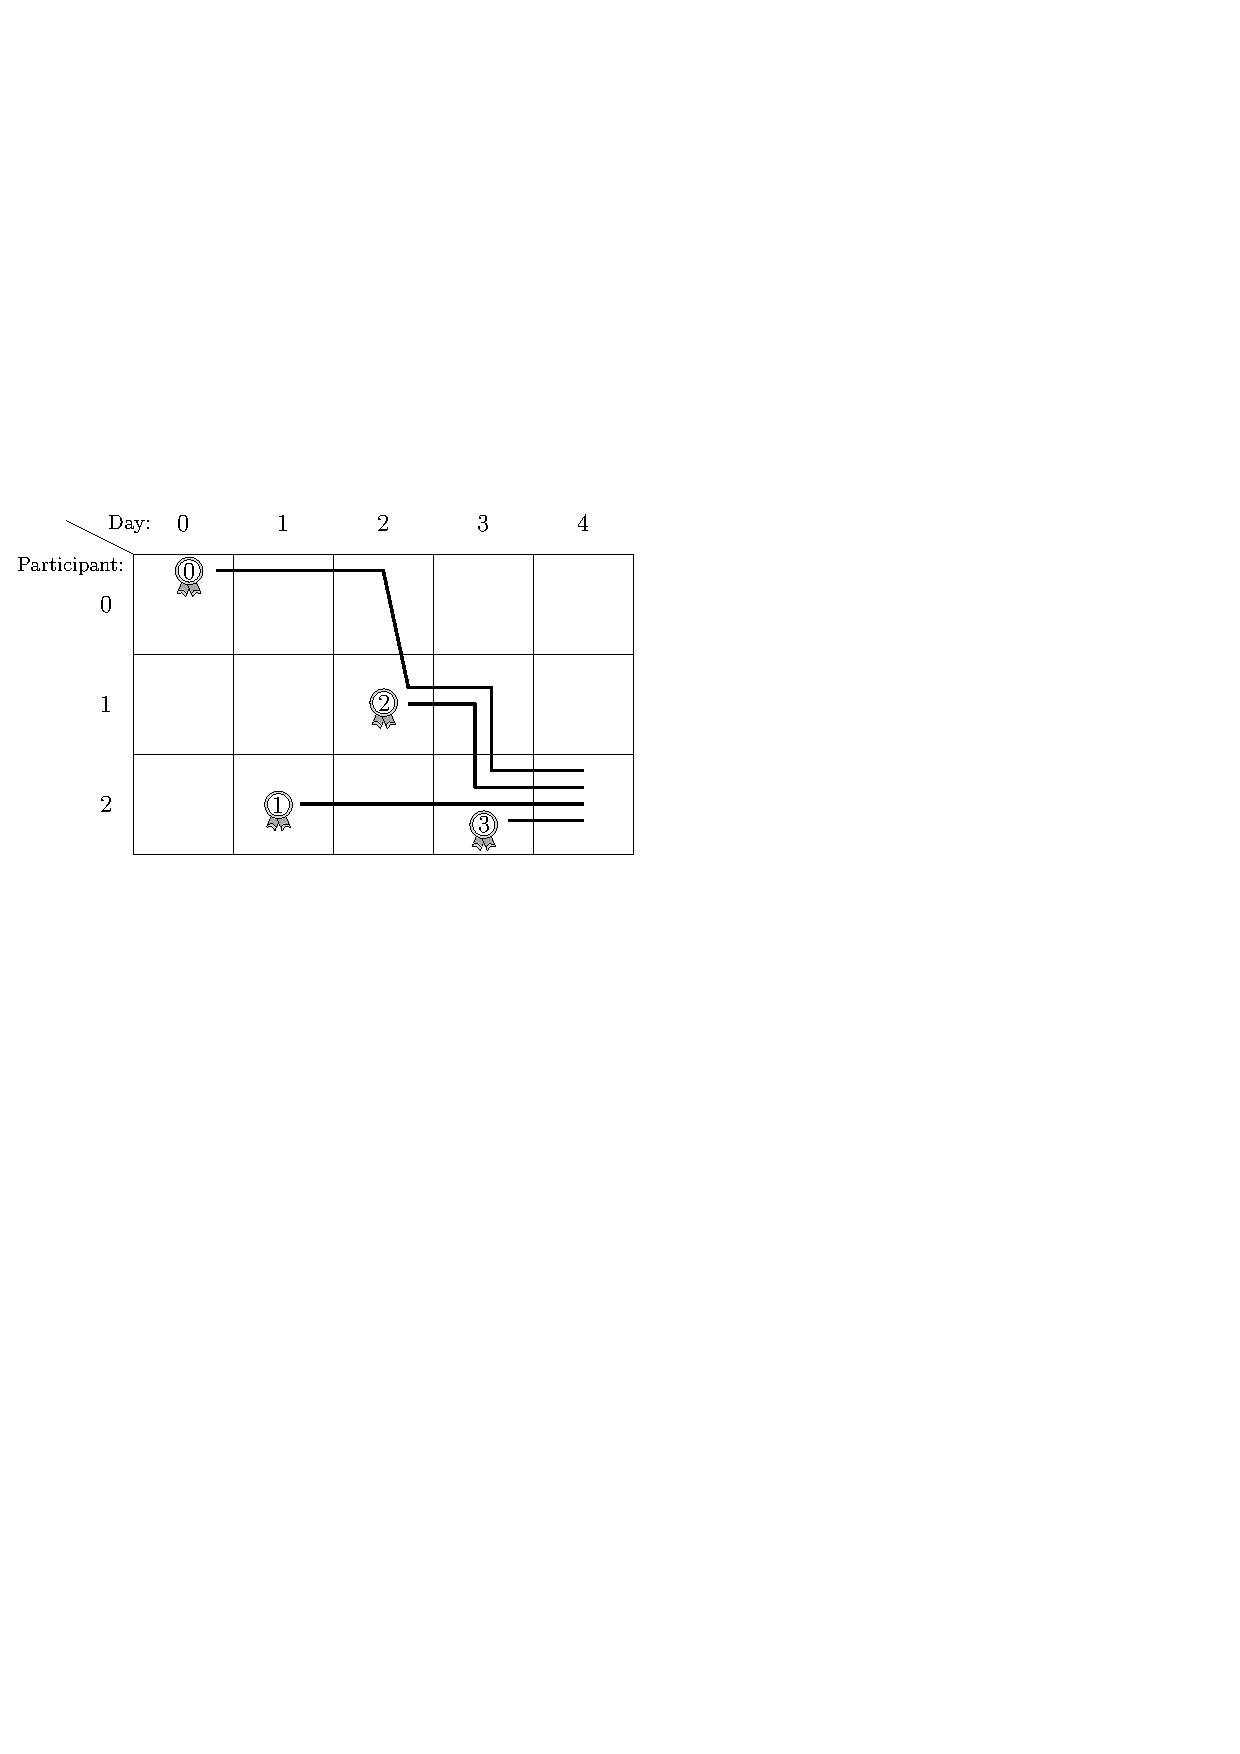
\includegraphics{sample-small}
\end{center}
\end{figure}
\vspace{1em}

The second sample can be seen below.

\vspace{1em}

\begin{figure}
\begin{center}
  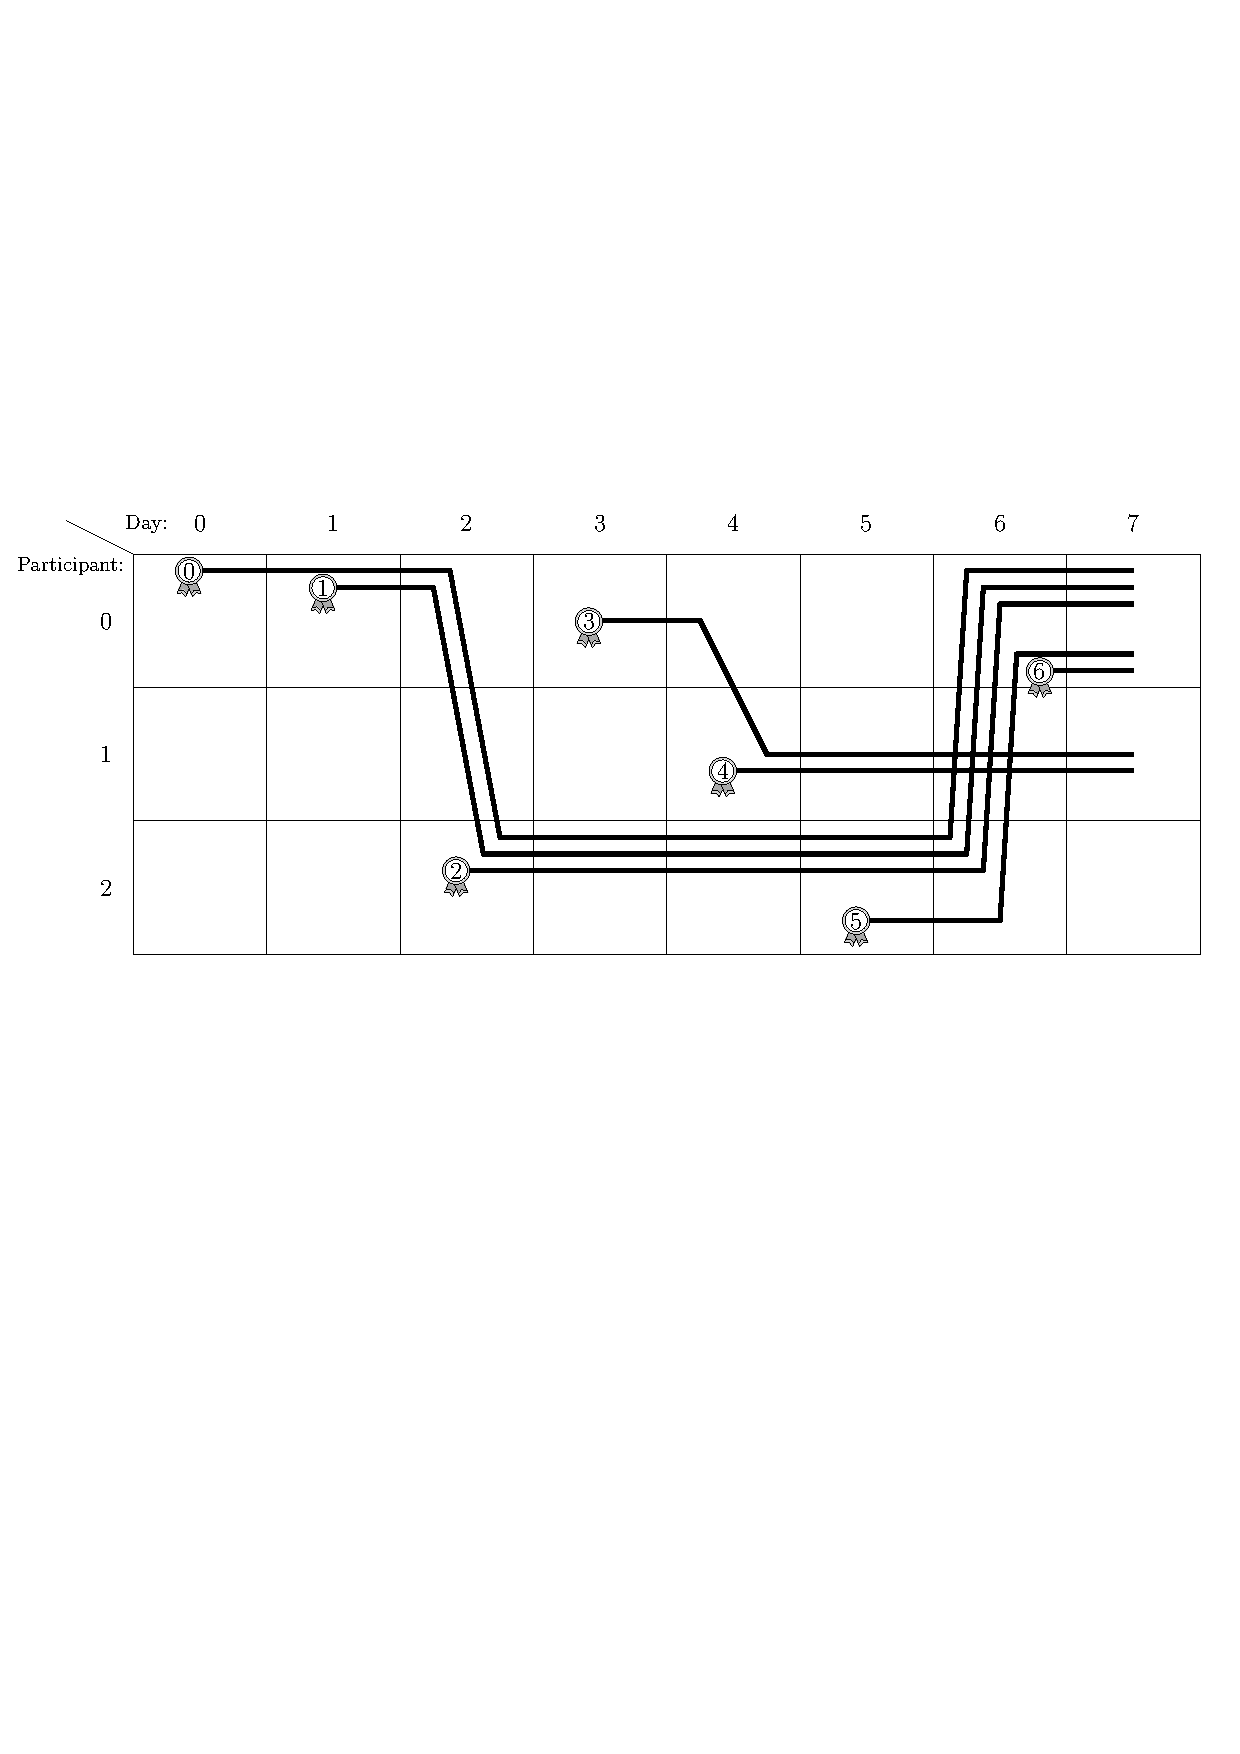
\includegraphics{sample_illustration}
\end{center}
\end{figure}

After the prize ceremony, participant 0 is given medals 5 and 6,
participant 1 is given medals 3 and 4, and participant 2 is given medals 0, 1 and 2.

